\documentclass[10pt]{article}
\usepackage{icmlko}

\icmlmeta{IP 파운데이션 월드모델}{266}{기록됐다는 사실이 신호로 새 들어왔다}{안 쓴 자료를 아홉 도메인에서 훑었더니 하나가 통과했고, 갈라 보니 내 절차가 만든 것이었다}

\begin{document}

\twocolumn[
\icmlheader

\begin{abstract}
노트 265가 유보 안 CV 나침반을 은퇴시키면서 살아 있는 것으로 ``안 쓴 자료
훑기''를 남겼다 --- 노트 255 · 260의 두 이득이 다 거기서 나왔다. 아홉
도메인의 레코드 필드를 축이 쓰는 것과 대조해 안 쓴 것을 전부 뽑았다(웹툰 5 ·
애니 10 · 모바일 7 · 게임 9 · 도서 6 · 펀딩 8 · 만화 8 · 세계애니 10).
잴 수 있는 후보 넷을 골랐다 --- 애니 \textbf{방영 분기}(몫 23.2\%) ·
세계애니 \textbf{제작사 이름}(11.7\%, 지금은 제작사 \emph{수}만 쓴다) ·
게임 \textbf{무료 여부} · 도서 \textbf{장르}. \textbf{하나가 통과했다}: 애니
방영 분기의 성분 3 이 연도 통제 $+$0.285 · 조각 5/5 · 겹침 0.229 로 노트
239 · 256의 검사 셋을 다 넘었다. 웹툰 태그($-$0.259)보다 세다. \textbf{갈랐다}
--- 성분 3 은 네 분기에 걸린 무게가 전부 $\approx -0.5$ 로 ``분기가 \emph{있나}''
방향이고, ``기록됨''과 $-$0.63 이다. 기록률이 학습 81.7\% 대 유보 93.6\% 로
다르고 그 ``기록됨''이 학습 라벨과 $+$0.342 다. \textbf{기록된 행 안에서만
다시 재니 네 성분이 전부 $|\rho| < 0.07$} --- 신호가 통째로 결측 무늬였다.
원인은 자료가 아니라 \textbf{내 절차}다: 토큰이 하나도 없는 행이 전부 0 이라
중심을 뺀 뒤 ``기록됐나''라는 방향을 만든다. 관측된 행으로만 중심잡고 적합하도록
고치니 \textbf{넷 다 통과 없음}이다. 이미 채택한 축들은 덮음이 100\% ·
99.8\% 라 안 걸린다(확인했다). \textbf{노트 264와 같은 병에 두 번째로
걸렸다} --- 그때는 가드가, 이번엔 후보 검사가 \emph{모형이 안 보는 값}으로
판정했다.
\end{abstract}
]

\section{살아 있는 나침반 하나}

노트 265가 유보 안 CV 여지를 은퇴시켰다(음수가 됐다). 남은 것 중 실적이 있는
것은 ``안 쓴 자료 훑기''뿐이다 --- 노트 255(웹툰 태그 내용)와 노트 260(웹툰
요일 · 등급 · 작가 수)이 거기서 나왔다.

이번엔 도메인 하나가 아니라 아홉을 한꺼번에 훑었다. 레코드 필드를 뽑아
그 도메인의 \texttt{*\_axes.py} 소스에 이름이 나오는지로 걸렀다.

\begin{center}\small
\begin{tabular}{lrl}
\hline
도메인 & 안 쓴 필드 & 눈에 띄는 것 \\
\hline
애니 & 10 & \texttt{air\_quarter} · \texttt{genres} \\
세계애니 & 10 & \texttt{studio\_name} · \texttt{source} \\
게임 & 9 & \texttt{is\_free} · \texttt{n\_dlc} \\
펀딩 & 8 & \texttt{category\_name} · \texttt{n\_delivery} \\
만화 & 8 & \texttt{genres} · \texttt{format} \\
모바일 & 7 & \texttt{advisory} · \texttt{n\_device} \\
도서 & 6 & \texttt{genre} · \texttt{pages} \\
웹툰 & 5 & (이미 다 썼다) \\
\hline
\end{tabular}
\end{center}

사후인 것(\texttt{avg\_rating} · \texttt{favourites} · \texttt{is\_ending} ·
\texttt{n\_episode})과 라벨 자신(\texttt{amount} · \texttt{y\_positive})을
빼고, 몫과 그럴듯함으로 넷을 골랐다.

\section{하나가 통과했다}

\begin{center}\small
\begin{tabular}{llrrr}
\hline
후보 & 성분 & 연도 통제 & 조각 & 겹침 \\
\hline
\textbf{애니 방영 분기} & \textbf{3} & $\mathbf{+0.285}$ & \textbf{5/5} &
  \textbf{0.229} \\
세계애니 제작사 & --- & \multicolumn{3}{c}{통과 없음} \\
게임 무료 여부 & --- & \multicolumn{3}{c}{조각이 안 돈다(학습 259)} \\
펀딩 카테고리 & --- & \multicolumn{3}{c}{토큰 1종} \\
\hline
\end{tabular}
\end{center}

$+$0.285 는 웹툰 태그($-$0.259)나 애니 태그($+$0.248)보다 세다. 검사 셋을
다 넘었으니 채택할 참이었다.

\section{갈랐다}

노트 133의 규칙 --- 첫 양수를 그대로 채택하지 않는다. 성분 3 에 무엇이
실렸는지 봤다.

\begin{center}\small
\begin{tabular}{lrrrr}
\hline
성분 3 무게 & 1분기 & 2분기 & 3분기 & 4분기 \\
\hline
 & $-$0.510 & $-$0.505 & $-$0.506 & $-$0.478 \\
\hline
\end{tabular}
\end{center}

\textbf{네 분기에 똑같이 걸려 있다.} 이것은 ``어느 분기냐''가 아니라
``분기가 \emph{있냐}''는 방향이다. 설명력도 5.8\% 로 앞 셋(35.9 · 29.5 ·
28.8\%)과 자릿수가 다르다.

\begin{figure}[t]
\centering
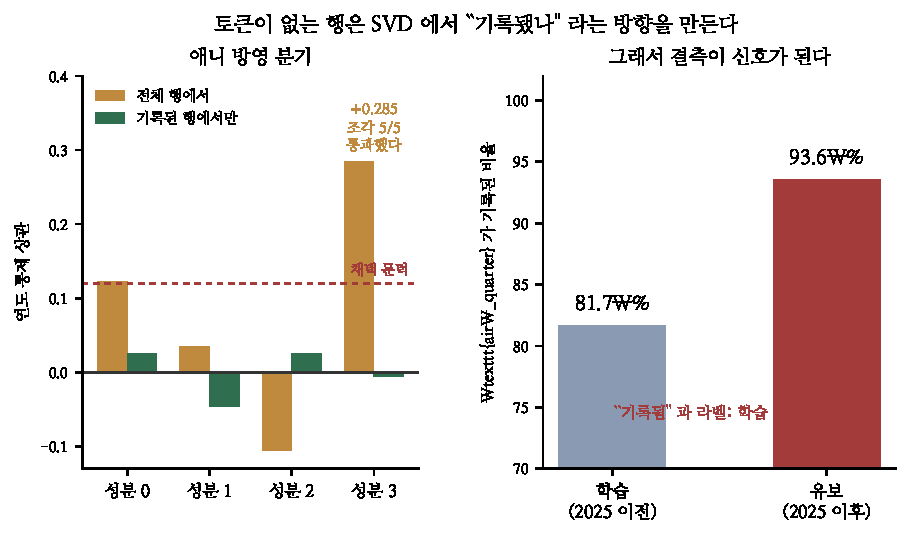
\includegraphics[width=\columnwidth]{figs/rec.pdf}
\caption{왼쪽 --- 전체 행에서 잰 것과 기록된 행에서만 잰 것. 오른쪽 ---
기록률이 시기마다 다르다.}
\end{figure}

\begin{center}\small
\begin{tabular}{lr}
\hline
성분 3 과 ``분기가 기록됨'' & $-$0.63 \\
기록률 (학습) & 81.7\% \\
기록률 (유보) & \textbf{93.6\%} \\
``기록됨'' 과 라벨 (학습) & $\mathbf{+0.342}$ \\
\hline
\end{tabular}
\end{center}

그리고 결정적으로 --- \textbf{기록된 행 안에서만} 네 성분을 라벨과 견주면

\[ -0.011,\quad -0.054,\quad -0.014,\quad -0.070. \]

\textbf{전부 0 근처다.} 방영 분기 자체는 아무것도 안 나른다. 실제 분기별
라벨 편차도 1분기 $+$0.187 부터 4분기 $+$0.065 까지 폭 0.12 로, 웹툰
요일의 0.41 과 견줄 것이 못 된다.

\section{자료가 아니라 절차가 만들었다}

기전이 단순하다. 토큰이 하나도 없는 행(분기 미기록 15\%)은 설계행렬에서
\textbf{전부 0}이다. 학습 전체로 중심을 빼면 그 행들이 다른 모든 행과
반대 방향으로 튀고, SVD 가 그것을 한 성분으로 잡아낸다. \textbf{내가 만든
성분이 결측 지표였다.}

관측된 학습 행으로만 중심잡고 적합하도록 고쳤다.

\begin{center}\small
\begin{tabular}{lrr}
\hline
애니 방영 분기 & 전체 행 & 기록된 행만 \\
\hline
성분 0 & $+$0.123 & $+$0.026 \\
성분 1 & $+$0.035 & $-$0.046 \\
성분 2 & $-$0.105 & $+$0.025 \\
\textbf{성분 3} & $\mathbf{+0.285}$ & $\mathbf{-0.006}$ \\
\hline
\end{tabular}
\end{center}

\textbf{넷 다 통과 없음}이 됐다. 세계애니 · 게임 · 도서도 마찬가지다.
\textbf{이번 훑기의 수확은 축 0 개다.}

\paragraph{이미 채택한 것은 안 걸린다} 확인했다 --- \texttt{tag\_c1\_웹툰} ·
\texttt{tag\_c3\_웹툰} · \texttt{meta\_c0\_웹툰} · \texttt{meta\_c3\_웹툰} 이
덮음 100\%, \texttt{tag\_c2\_애니} · \texttt{tag\_c3\_애니} 가 99.8\% 다.
토큰 없는 행이 사실상 없어 그 방향이 안 생긴다. 고친 뒤 판이 0.4842에서
0.4839 로 넷째 자리만 움직인다(애니 네 행).

\section{두 번째로 같은 병}

노트 264에서 새로 만든 가드가 \textbf{모형이 안 보는 값}(이미 마스크 0 인
86\%)으로 판정했고, 노트 187의 값싼 검사가 잡았다. 그때 이렇게 적었다 ---
``가드는 축을 검사하는 코드지 검사에서 면제된 코드가 아니다.''

\textbf{이번엔 후보 검사가 같은 짓을 했다.} 마스크가 0 이 될 행을 넣고
성분을 만들었다. 두 번 다 ``관측된 행에서만 읽는다''를 안 지킨 것이고,
두 번 다 \emph{내가 새로 쓴 코드}에서 났다. 오래된 코드는 그 규칙을 지키고
있었다(\texttt{forms.\_feat} 이 마스크로 중립 대입을 한다).

\paragraph{남은 것}
\begin{center}\small
\begin{tabular}{ll}
\hline
갈래 & 왜 \\
\hline
훑기가 비었다 & 아홉 도메인에 남은 자료가 없다는 뜻인가 \\
덮음 낮은 후보 & 55$\sim$85\% 짜리는 절차상 못 쓰나 \\
\texttt{SOURCE} 채우기 & 20/45 쌍 \\
라벨 자체 & 노트 209 --- 축은 다 훑었다 \\
\hline
\end{tabular}
\end{center}

\paragraph{규약} 후보를 만들 때도 \textbf{관측된 행에서만} 중심잡고 적합한다.
덮음이 100\% 가 아닌 필드는 결측이 성분 하나를 통째로 차지할 수 있고, 그
성분은 검사 셋을 \emph{통과한다} --- 연도 통제도 조각 부호도 겹침도 다.
결측은 신호처럼 생겼다.

\end{document}
